\documentclass[twoside,a4paper,12pt]{article}

\usepackage{graphicx}
\usepackage{url}
\usepackage{verbatim}
\usepackage{pgfplots}
\pgfplotsset{compat=1.11}
\usepackage{tikz}
\usetikzlibrary{positioning}
\usepackage{amsmath}
\usepackage{amsfonts}
\usetikzlibrary{arrows,shapes,positioning,shadows,trees,er}
\usepackage{color}
\usepackage{listings}
\usepackage{hyperref}
\usepackage[xindy]{glossaries}
\usepackage{todonotes}
\makeglossaries
\title{ Building and evaluating a multimodal co-occurence-based recommender engine with Apache Mahout and Apache Solr }
\author{
	Author \\
	Lukas Hofmaier \\
	lukas.hofmaier@hsr.ch
 	\and
	Supervisor \\
        Hansj\"org Huser \\
        hansjoerg.huser@hsr.ch
}
\date{
	\textsc{University of Applied Sciences Rapperswil}\\
	Project Thesis,
	\today
}


\newglossaryentry{topn}
{
name=top-N recommendations list,
description={The recommender engine suggest $N$ specific items that are likely appealing to him. This 'best bet' is called top-N recommendation list}
}

\newglossaryentry{indicator}
{
name={indicator},
plural={indicators},
description={Indicator are Item ID associated with a particular item. Indicators are derived from user actions. They lead to other items that are recommendable for the same action. For example if you wish a user to purchase something and you collect all users purchase interactions you can create purchase indicator for every item based on these interactions}
}

\newglossaryentry{coocc}
{
name={co-occurence},
description={Co-occurence in the context of user-item interactions describes the number of shared users that interacted with a two particular items. Co-occurence can be interpreted as an indicator of similiarity between the two items}
}

\newglossaryentry{tag}
{
name={tag},
plural={tags},
description={A tag is a non-hierarchical keyword or term assigned to an item (e.g. movie). It describes an item and allows it to be found again by browsing or searching. Tags are generally chosen informally and personally by users who visit an item}
}

\newglossaryentry{scalable}
{
name={scalable},
description={Scalability is the ability of a system, network, or process to handle a growing amount of work in a capable manner or its ability to be enlarged to accommodate that growth}
}

\newglossaryentry{multimodal}
{
name={multimodal},
description={Multimodal interaction means that the user can interact in multiple modes with a system}
}

\newglossaryentry{precision}
{
name={precision},
description={Precision is the fraction of retrieved instances that are relevant}
}

\newglossaryentry{recall}
{
name={recall},
description={recall (also known as sensitivity) is the fraction of relevant instances that are retrieve}d 
}

\newglossaryentry{preference}
{
name={preference},
plural={preferences},
description={A preference is the association of a user and an item and a number expressing the strength of the user's preference for the item}
}

\newglossaryentry{llr}
{
name={log-likelihood},
description={The log-likelihood ratio is a probabilistic measure of the importance of a co-occurrence}
}

\newglossaryentry{indicatorm}
{
name={indicator matrix},
description={An indicator matrix is an $n \times n$ matrix where the values are log-likelihood ratio strengths of the co-occurences}
}

\newglossaryentry{like}
{
name={like},
plural={likes},
description={A like is a positive feedback of a user associated with an item. The user interface provides a button to like an item}
}

\newglossaryentry{useraction}
{
name={user action},
plural={user actions},
description={A user action describes the interaction of a user with the GUI. Examples are: view, purchase, like }
}
\newglossaryentry{rec}
{
name={co-occurence based recommender},
description={An itembased recommender engine that uses log-likelihood ratio of co-occurences of items in the users action history. It uses a search engine to produce recommendations. The query for the search engine are formed from the user's history }
}

\newglossaryentry{rankedretrieval}
{
name={ranked retrieval},
description={Ranked retrieval is the process of sorting document by their relevance to a query. The most relevant document are listed first}
}

\begin{document}

\lstset{
basicstyle=\ttfamily\footnotesize,
columns=fullflexible,
keepspaces=true,
captionpos=b
}

\maketitle
\tableofcontents

\begin{abstract}
Building a recommendation engine can be a difficult and expensive task. Understanding all possible techniques and choosing the most suitable for the job at hand presupposes that you have a strong mathematical background. There are a lot different algorithms and strategies and researchers are constantly coming up with new ones. Not all companies can afford to employ an army of data scientist and mathematicens to build a recommender system. They a have to trade-off the accuracy of recommender against the development costs. 

This report describes a simple pratical approach to build a recommender system that is more approacable for small development teams. 
In order to produce a list of recommendable items for a user instantly, it uses the user' history of recent actions to query the search engine Apache Solr for similar items. 
Similarity among items is based on the \gls{llr} ratio of co-occurences of several action types (e.g. purchase, view). 
This approach exploits existing and proved technologies to save development costs. 
Further the system is scalable for big data because Solr is optimized for to search large volumes of data and co-occurence can be computed at scale with Apache Mahout's \verb|spark-itemsimilarity| job.

This report explains the core concepts of this practical approach on the basis of a small demo web applicatoin. It will explain the similarities between the weighting of indicator scores of a this model and the process of ranked retrieval.

The evaluation of the described approach shows that the accuracy of the top-N recommendation task matches the accuracy of a sophiticated itembased algorithm.
\end{abstract}

\section{Introduction}
\label{sec:intro}

Recommender systems help consumers to discover unknown articles from an overwhelming set of choices by suggesting them a list of items that are likely to be appealing to them. The recommended items should match the user's personal taste.

For instance, they help users of an on-demand movie provider to find previously unknown and interesting movies. Such a provider may offer 100'000 different titles. It is not feasible for a user to check every movie separately in order to decide if he likes it or not. A recommender engine supports users by presenting them a list of movie recommendations. It predicts the user's \gls{preference} for each movie and shows him a list of movies with the highest predicted score. The list of recommendations is referred to as \gls{topn}. For example, if a user has purchased the movies "Terminator 2" and "Transformers" the recommender engine might present him a list of other similar action movies like ``Matrix'' or ``Iron Man''. 
 
Recommender systems have become very common in recent years. E-commerce sites that deploy a recommender engine can have an increase in sales of 8-13 percent.\footnote{http://www.practicalecommerce.com/articles/1942-10-Questions-on-Product-Recommendations}

\subsection{Overview of recommender strategies}
\label{sec:strategies}

A trivial solution to the recommender problem would be to sort all items by their popularity or average rating in descending order and then suggesting the user the top $N$ items of that sorted list. Recommender systems based on this approach are called non-personalized. Non-personalized \glspl{topn} do not involve computationally expensive procedures and are easy to implement but they suggest all users the same items. The web site www.imdb.com is an example for a non-personalized recommender. It shows the user a list of movies sorted by the average rating score.
 The recommender described in this report is a personalized recommender that creates an individual list of recommendation for every user.

There are different strategies to create personalized \glspl{topn} \cite{jannach11}. Figure \ref{fig:overview} shows an overview of some possible techniques.

\tikzset{
  basic/.style  = {draw, text width=3cm, drop shadow, font=\sffamily, rectangle},
  root/.style   = {basic, rounded corners=2pt, thin, align=center,
                   fill=green!30},
  level 2/.style = {basic, rounded corners=6pt, thin,align=center, fill=green!60,
                   text width=8em, edge from parent/.style={->,draw,color=black},>=latex},
  level 3/.style = {basic, thin, align=left, fill=pink!60, text width=8.5em}
}
\begin{figure}
  \centering
\begin{tikzpicture}[
  level 1/.style={sibling distance=50mm},
  edge from parent/.style={->,draw},
  >=latex]

% root of the the initial tree, level 1
\node[root] {Recommender strategy}
% The first level, as children of the initial tree
  child {node[root] (c1) {Non-personalized}}
  child {node[root] (c2) {personalized}
    child {node[level 2] (c21) {Collaborative filtering}
      child {node[level 2] (c2111) {Neighborhood based}}
      child {node[level 2] (c2112) {Latent factor approach}}}
    child {node[level 2] (c22) {\gls{content} filtering}}};
  
% The second level, relatively positioned nodes
\begin{scope}[every node/.style={level 3}]

\node [below of = c2111, xshift=15pt] (c211) {Pearson Correlation};
\node [below of = c211] (c212) {Cosine similarity};
\node [below of = c212] (c213) {LLR ratio};

\node [below of = c2112, xshift=15pt] (c21121) {Gradient descent};
\node [below of = c21121] (c21122) {Least Square};

\end{scope}

% lines from each level 1 node to every one of its "children"

\foreach \value in {1,...,3}
  \draw[->] (c2111.195) |- (c21\value.west);

\foreach \value in {1,...,2}
  \draw[->] (c2112.195) |- (c2112\value.west);

\end{tikzpicture}
    \caption{Overview of some common recommender strategies}
\label{fig:overview}
\end{figure}


\begin{description}
\item[Collaborative Filtering] This strategy is only based on past user behavior. Such behavior include explicit user ratings or other user activities like purchases, likes and clicks. For example, a recommender engine based on collaborative filtering uses the ratings of all users to compute the similarity between all items. 
It requires no domain knowledge. Recommender engines based on collaborative filtering do not care what the items are and what attributes they have. This can be an advantage because the same technique can be applied to different domains and different types of items. 

User preferences will change over time. Another advantage is that collaborative filtering will update the model automatically as it is exposed to new user histories. The systems learns.
Further collaborative filtering algorithms can be divided in two different approaches.
\begin{description}
\item[Neighborhood based] Neighborhood models are based on the similarity among users or items. For instance, two items are similar because they have similar ratings of the same users. The set of items that are similar to a particular item $i$ is called the neighborhood of $i$. In order to predict a unknown preference for an item $i$ the recommender computes the nearest neighbors of $i$ and considers the users past ratings for the similar items. This approach was used by Amazon.com according to \cite{Linden}. Neighborhood models can be further divided by their similarity metric (e.g. cosine, log-likelihood ratio).
\item[Latent factor approach] Latent factor approaches model users and items as vectors. The rating of a user on an item is predicted by computing the inner product between the related latent factor vectors. The recommender problem is reduced to the optimization problem of finding the best vectors with respect to a training set.
\end{description}
\item[\gls{content} filtering] \gls{content} recommendation techniques use attributes of items in order to predict preferences of users. For example, a movie can be described by \glspl{tag}. A user profile indicates the type of items a user likes. These algorithms recommend items that are similar to the user profile. The profile could be built from the user's past actions.
\end{description}

This report describes a personalized recommender that uses a combination of collaborative filtering and content-based filtering. In order to compute similarities among items it uses both; past user actions and \glspl{tag} associated with items. Hence it is a hybrid recommender system.

\subsection{Why is it difficult to build a recommender engine?}

To make a rationally choice which strategy to use for the job at hand is difficult and requires a strong mathematical background. According to \cite{Dunning14} the process of designing an advanced and accurate recommender engine requires a team of highly trained engineers and data scientists. The process requires to try a huge collection of algorithms for each problem and selecting the algorithm that gives the best result. This is too expensive for small companies. Apart from choosing the strategy there are several other challenges in building a recommender engine.

\begin{itemize}
\item Collaborative filtering algorithms are based on collecting a large amount of past user preference data. Most techniques use explicit user ratings. For instance, users are invited to rate items on a scale from 1 to 5. Only a small subset of users rate a small subset of items. This leads to very few ratings and these ratings represent only users who like to rate.

\item When dealing with huge data sets, the calculation of the similarities or the latent factor vector is computationally expensive. Either a large amount of computation power is necessary or the computation of a \gls{topn} takes too long.
\end{itemize}

\subsection{The design goals of a practical recommender}
\label{sec:practical}

In order make the development of a recommender engine easier and cost-effective Ted Dunning  proposes in \cite{Dunning14} a simplified, practical approach that provides profitable results and facilitate the processing of large-scale data sets. 

The design proposed by \cite{Dunning14} has the following goals:
\begin{itemize}
\item A small-scale development teams can build a recommender engine.
\item To build the model, the systems uses algorithms that can be computed at scale with a distributed computation framework, such as Apache Hadoop or Apache Spark. 
\item The \gls{topnt} should be fast. Recommendations are generated instantly and online. Computation of similarity and the update of the text search engine is done offline, ahead of time.
\item Use input data that reveals what user want to do. The quality of a recommender depends on the input data that is used to build the model (train the recommender). 
\item Several types (e.g. clicks, views, purchases) of user actions are used to improve recommendations and it is possible to extend the recommender with additional \glspl{indicator}. Many existing collaborative filtering algorithms use only one user activity to model preference \cite{ferrel}. In addition meta data, like \glspl{tag}, are used to improve the accuracy. A recommender that uses a variety of user activities is called a \gls{multimodal} recommender. 
\end{itemize}

To achieve these goals Ted Dunning makes the following suggestions in \cite{Dunning14}.

\begin{itemize}
\item The recommender engine takes user behavior instead of explicit user ratings as input. Because only a small subset of users are willing to rate items and user behavior is the best clue to what they want. Hence the input data should consist of collected user behavior, like clicking or purchasing.

\item Use \gls{coocc} as an \gls{indicator} for similarity. Co-occurrence counts how many times two items appear together in user histories. Among others there are two reason to use \gls{coocc}. 

\begin{itemize}
  \item User behavior interaction are only associations between a user and an item and there is no notion of the association's strength represented as number. This associations are Boolean preferences. It exist or it doesn't exist. Co-occurrence is suitable for Boolean preferences because it does not account for a strength of the interaction. In addition, it can be used to analyze every type of interaction. For instance, we can also count \gls{coocc} of items associated with tags.
  \item Co-occurrence can be computed using the \gls{mapreduce} programming model. Hence the computation of the model can be distributed.
\end{itemize}

\item Use a text retrieval engine to produce the \gls{topn}. Producing a \gls{topn} with a neighborhood based collaborative filtering algorithm is similar to process a document query in a text retrieval system. Because a \gls{rankedretrieval} is a way of finding similar documents according to a query we can use \gls{rankedretrieval} to find similar items to the ones the user already expressed some interest.
 We use similarity indicators based on \gls{coocc} to score every item that matches the query.
The search engine indexes items represented as documents instead of text documents. The fields of these documents contain similar items. The query is composed of items that are associated with the user's past actions which we want to recommend. For instance, if we want to recommend items which the user can purchase then we use his purchase history. 

It is possible to store several indicators as fields within a document of the search engine. Hence we can use many types of user actions to improve recommendations. For instance we can use one field that indicates similarity with respect to purchases and one field that indicate similarity with respect to \glspl{tag}. In addition we can enhance the index with meta data about the items.

We exploit the search capabilities of an existing text retrieval engine, such as Apache Solr. This saves development costs. In addition the system is \gls{scalable} for big data because Solr is optimized to search large volumes of data.

\end{itemize}

There are academic approaches that produce recommendations with a smaller error but these require complex mathematical models. The focus of this approach is not to minimize the error but to make the development and deployment of a recommender more approachable. Another difference is that the described recommender does not predict a rating value for every item for every user. Instead it suggests the user a \gls{topn}.


\subsection{Used technology}
\label{sec:tech}

In order to illustrate the concepts by example, we build a small demo web application that implements a \gls{rec} with a search engine. Users can browse a movie database. They can express their preference with a ``like'' button associated with every movie. In addition they can tag movies. Users can click on the discover link and the web application will present them a list of recommended movies. A large amount of functionality is provided by two existing technologies.

\begin{itemize}
\item Apache Mahout
\item Apache Solr
\end{itemize}

Apache Mahout is a top-level Apache project that exists since 2008. Among other machine learning techniques it implements a number of collaborative filtering algorithms. It is also \gls{scalable}. Some algorithms run on top of Apache Spark or Apache Hadoop in order to process large amount of data\cite{Owen}. We used it because it provides a job to compute the \gls{llr} ratios of \gls{coocc} and because it is well documented.

Apache Solr is a search engine that is optimized to search large volumes of text-centric data and it returns results sorted by relevance. It is built on Apache Lucene, an information retrieval library \cite{grainger}.

\subsection{Overview}
The report is split into three parts.
In section \ref{sec:design} we present the core concepts of the co-occurrence based recommender. First we describe the used input data. Then we explain the process of computing a \gls{topn} and the \gls{coocc} based similarity metric. In the next section we describe the similarities of a text-retrieval engine to a recommender and how we map items to text documents.

In section \ref{sec:integration} we show how to connect the building blocks described in the previous sections.

In section \ref{sec:evaluation} we evaluate the accuracy of the \gls{rec}. We describe appropriate performance metrics, \gls{precision} and \gls{recall}, for the top-N recommendations task (section \ref{sec:precision}). 
Then we explain the evaluation methodology (section \ref{sec:methodology}) and the baseline algorithms (section \ref{sec:baseline}). 
We use the rating and tag activity data of the MovieLens data set (section \ref{sec:dataset}) as an evaluation test set. 
Finally we present the results of the performance evaluation. 













\section{Core concepts of the \gls{rec}}
\label{sec:design}

In order to set a context we will first give a broad overview of how the discussed recommender computes a \gls{topn}.
The conceptual process can be divided into five steps. Figure \ref{fig:topndataflow} illustrates this simplified view.

\begin{enumerate}
\item A user requests a \gls{topn}.
\item The recommender looks up items that appear in the recent user history. The history contains multiple types of past user actions.
\item A query composed of items from the user's action history is sent to the search engine.
\item The search engine returns a ranked search result set of items according to the query. Because a \gls{rankedretrieval} is a way of finding similar documents according to a query we can use \gls{rankedretrieval} to find similar items to the ones the user already expressed some interest.
 We use similarity indicators based on \gls{coocc} to score every items that matches the query.
\item The recommender removes items already known to the user and presents him a \gls{topn}.
\end{enumerate}

\tikzset{
  reco/.style={
    draw, text width=3cm,drop shadow,font=\sffamily, rectangle,rounded corners=2pt,thin,
    align=center,fill=green!30
  },
hist/.style={reco, fill=blue!30
},
se/.style={reco, fill=red!30
}
}

\begin{figure}
  \centering
  \begin{tikzpicture}[->, >=latex]
    \node[reco] (rec) at(180:3cm) {Recommender};
    \node[hist] (hist) at(60:3cm){History};
    \node[se] (se) at(300:3cm){Search engine};
    \node (user) [left of=rec,node distance=5cm]{User};
    \node(x)[align=left] at(120:1.7cm){2. lookup\\ user's history};
    \node(x)[align=left] at(0:2cm){3. user's\\ history};
    \node(x)[align=left] at(220:4cm){4. ranked \\ search result};
    \draw[->, >=latex] (170:3cm) arc  (170:100:3cm);
    \draw[->, >=latex] (40:3cm)  arc (40:-40:3cm);
   \draw[->, >=latex] (250:3cm)  arc (250:190:3cm);
   \draw[->, >=latex] (40:3cm)  arc (40:-40:3cm);
   \path (user) edge[bend left=40] node[anchor=south,above] {1. request top-N list}(rec);
   \path (rec) edge[bend left=40] node[anchor=north,below]{5. top-N list}(user);
  \end{tikzpicture}
  \caption{The process of producing top-N recommendations list a can be divided into five steps}
  \label{fig:topndataflow}
\end{figure}

In this section we deal mainly with the step 4, the scoring of items with respect to a user's history.
A recommender needs some data in order to build a model, also called training data. 
First we describe the kind of training data used by the \gls{rec}. 
Then we explain how the \gls{topn} is computed in theory and why we use the \gls{llr} ratio of \glspl{coocc} as a similarity metric.
Next we show the similarities of the \gls{topnt} and a \gls{rankedretrieval}, how we map items to documents stored in Solr and how we extend Solr's scoring function to match our needs.

\subsection{Record user behavior}
\label{sec:inputdata}

\begin{figure}
  \centering
     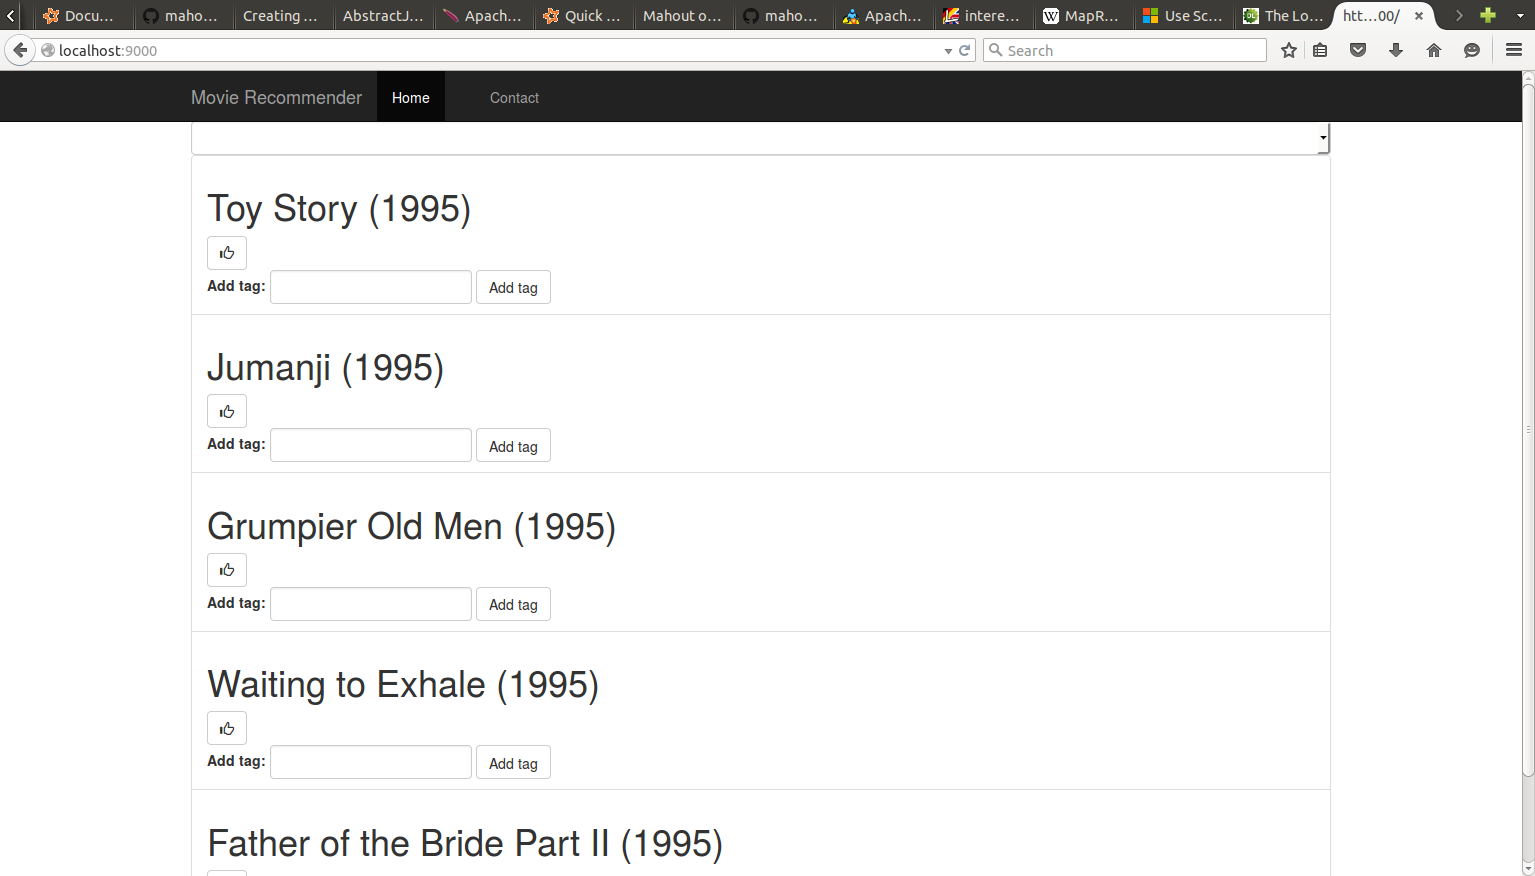
\includegraphics[width=0.9\textwidth]{collectinginput}
  \caption{The user can like and tag movies with the web front end. The user actions are recorded by the web server.}
  \label{fig:gui}
\end{figure}

The \gls{rec} suggests items that are similar to the ones the user already liked in the past. In order to build a model for similarity we need to train the recommender with some data about the items.
This section will descibe the type of input data we use  in our demo application. The report will refer to this type of input data. 

Many collaborative filtering recommender engines use excplicit user ratings to train their model. Explicit user ratings of a user for an item are expressed by numbers (e.g. a rating is a number between 1 and 5). The use of explicit feedback has some drawbacks.
\begin{itemize}
\item Only a small subset of users will rate items. This leads to a model that is skewed against user who like to rate.
\item The majority of ratings are associated with a small fraction of the most popular items \cite{Anderson}. As a result it is less likely that unknown items show up in the \gls{topn}. This behavior is undesirable because the goal of the recommender is to present items the a user would not find on his own.
\end{itemize}


Corresponding to \cite{Dunning14} the best choice of input data is the history of what a user actually does on a website. Hence the input data should consist of recorded \glspl{useraction} (e.g. purchase, view, like, tag).

In our demo web application we record two different user actions:
\begin{description}
\item[like]  Users can express their positive feedback for a movie by clicking on a ``like'' button (the \gls{like} action is an explicit rating. We use it instead of a purchase or view action in order to keep the GUI simple).
\item[tag] User can \gls{tag} items. Every item can be associated with a list of \glspl{tag}.
\end{description}
The recorded like and tag action are later used to compute similarity between items.
Figure \ref{fig:gui} shows the simplistic user interface of our demo web app.

The web browser sends every user action to the web server. The web server provides a REST Web API that receives the \glspl{useraction} as HTTP \verb|Post| request and saves them to a sqlite3 \footnote{https://www.sqlite.org/} database.

In order to analyse the data later we want to retrieve the action history $h_u$ for a particular user $u$ for a defined action and a list of tags for every item. Hence we have to structure the data accordingly. Figure \ref{fig:er} shows the entity relationship diagram for the user actions \gls{like} and \gls{tag}

\tikzset{multi  attribute/.style={attribute ,double  distance=1.5pt}}
\tikzset{derived  attribute/.style={attribute ,dashed}}
\tikzset{total/.style={double  distance=1.5pt}}
\tikzset{every  entity/.style={draw=blue , fill=blue!20}}
\tikzset{every  attribute/.style={draw=yellow, fill=yellow!20, node distance=1.0cm}}
\tikzset{every  relationship/.style={draw=red, fill=red!20}}

\begin{figure}
\centering
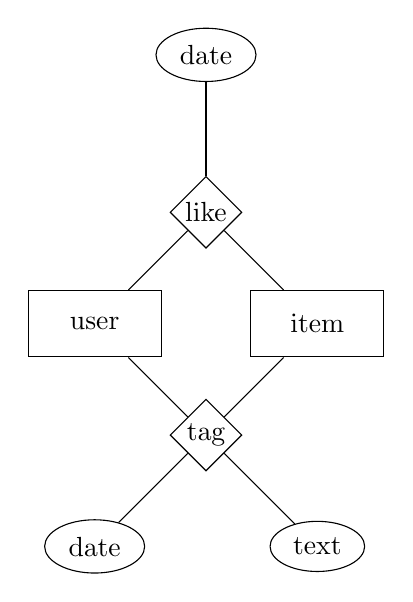
\begin{tikzpicture}[node distance=2.0cm]
  \node[entity](user){user};
  \node[relationship](like)[above right of=user]{ like } edge (user);
  \node[attribute](date2)[above of=like]{ date } edge (like);
  \node[entity](item)[below right of=like]{item} edge (like);
  \node[relationship](tag)[below right of=user]{ tag } edge (user) edge (item);
  \node[attribute](text)[below right of=tag]{ text } edge (tag);
  \node[attribute](date1)[below left of=tag]{ date } edge (tag);
  \end{tikzpicture}
\caption{The data model allows us to retrieve the action history for every user. Like and tag form associations of user with item.}
\label{fig:er}
\end{figure}

It makes sense to start recording behavioral data month's before depoying the recommender engine because the recommender engine has to analyze the data and build a model of similarty among items in order to create personalized recommendations.


\subsection{How to compute the top-N recommendations list?}
\label{sec:problem}
This section gives a mathematical description of the top-N recommendation task and hence it describes the computations required to produce recommendations. The description refers to the \gls{rec}.

Suppose we have a metric to express similarity between two items as a numerical value and the magnitude of the value determines the strength of similarity. If we compute the similarity for every item pair in a set of $n$ items, we can represent the result in a matrix $M$. $M$ is a $n \times n$ matrix. Each row and each column contains the similarities between one particular item and all other items. $M$ is symetric across the diagonal because the similarity between $a$ and $b$ must be the same as between $b$ and $a$ (commutativity). The diagonal of $M$ contains the value for maximum similarity because this value represents the comparison of an item to itself. $M$ is called the \gls{indicatorm}. Equation \ref{eq:similaritymatrix} shows an example of an \gls{indicatorm} with 4 items.

\begin{equation}
  \label{eq:similaritymatrix}
M =\bordermatrix{~ & 1 & 2 & 3 & 4 \cr
 1 & 1  & 0.40 & 0.9 & 0.1 \cr
2 & 0.40 &1  & 0.9 & 0.1 \cr
 3& 0.9 & 0.9 &1  & 0.63 \cr
 4 & 0.1 & 0.1 & 0.63 &1  \cr}
\end{equation}
Further we represent a user action history for each user as vector $h_l$ of length $n$. $h_l$ contains an element for every item. The user's interactions with an item are represented as binary values in $h_l$. If the there is an interaction with an item in the history the value or the corresponding element is 1. Otherwise the value is 0. For example equation \ref{eq:history} shows a user's action history for the action ``like''. He has liked item 1 and 2.

\begin{equation}
\label{eq:history}
h_l =
\begin{pmatrix}
 1 \\
 1 \\
 0 \\
 0 \\
\end{pmatrix}
\end{equation}

To create a \gls{topn} for user $u$ we compute the matrix vector product of $M$ and $h_l$. Equations \ref{eq:recommendation} actually means to compare the user history $h_u$ to the rows of the indicator matrix $M$. This result in a vector $r$ containing a score for each item that indicates the strength of the match (or similarity) of the item to the history $h_p$. The result $r$ is a vector of length $n$, that contains a score for every item. Hence $r$ maps every item to a value that indicates how likely an item is of interest to user $u$. According to equation \ref{eq:recommendation} item 3 correspond to the best recommendation.

\begin{align}
  \label{eq:recommendation}
r_u &= M h_u 
&=
\begin{pmatrix}
  1  & 0.40 & 0.9 & 0.1 \\
 0.40 &1  & 0.9 & 0.1 \\
  0.9 & 0.9 &1  & 0.63 \\
  0.1 & 0.1 & 0.63 &1 \\  
\end{pmatrix} 
\begin{pmatrix}
 1 \\
 1 \\
 0 \\
 0 \\
\end{pmatrix}
&= 
\begin{pmatrix}
 1.4 \\
 1.4 \\
 1.8 \\
 0.2 \\
\end{pmatrix}
\end{align}

In order to create the complete \gls{topn} based on the vector $r$ we create a list of all items sorted by thev alues in $r$. Items with a high value appear first in the list. Then we remove all items from the list the user hasn't seen (the ones with zeros in $h_u$). In other words we return a ranked list of items. This list forms the \gls{topn}. In the example of equation \ref{eq:recommendation} the recommender would return item 3 followed by item 4. Item 1 and to are removed because the apear in the user's history.

\subsection{How to measure similarity among items?}
\label{sec:llr}

In the last section (\ref{sec:problem}) we use a matrix $M$ that contains similarity strength among items. This section describes how $M$ is computed.

In order to compute the similarity between two items we count the \gls{coocc} among two items with respect to a particular user action and then compute the the \gls{llr} ratio of that \gls{coocc}.

\subsubsection{Co-occurence}
\label{sec:cooccurence}

Co-occurence in the context of a recommender system is the number of times a pair of items appear together in some user's action history. For instance, if there are 5 users who all liked items $A$ and $B$ then $A$ and $B$ co-occur 5 times. Coocurrence indicates similarity. The more two items turn up togheter, the more related they probably are. We can count the \gls{coocc} of items with respect to any action or entity. For instance, we can count how many times two items are associated with the same tag or purchased by the same users.

\subsubsection{Log-likelihood ratio}
\label{sec:llrs}

\gls{llr} is a probabilistic measure of the importance of a \gls{coocc}. The \gls{llr} similarity  is the probability that two users share the same items because the items are similar and not due to chance. It finds important \gls{coocc} and filters out the coincidental. Hence it avoids that the result is skewed against popular items \cite{Dunning93}. Compared to the Jaccard coefficient \cite{Hartung} the log-likelihood-based similarity computes higher similarites for anomalous co-occurences than for items that occur in every user history. For a detailed explanation of the math involved see appendix and \cite{Dunning93}. 

According to \cite{Dunning14} using the \gls{llr} ratio of the \gls{coocc} has several advantages.
\begin{itemize}
\item It yields good results for data that only captures the interaction and no \glspl{preference} \cite{Dunning93}.
\item The similarity is not skewed against popular items.
\item We can use distributed MapReduce based algorithms to compute the \glspl{coocc}. Hence the computation of the \gls{llr} similarity is \gls{scalable}.
\end{itemize}

\begin{figure}
\centering
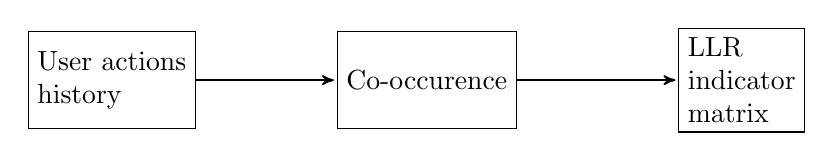
\begin{tikzpicture}[node distance=40mm,
data/.style={
rectangle,
draw,
thin,
minimum height=3.5em
},
to/.style={->,>=stealth',shorten >=1pt,semithick,font=\footnotesize},
]
\node (hist) [data, align=left] {User actions\\history};
\node (co) [data,right of=hist,align=left] {Co-occurence};
\node (in) [data,right of=co,align=left] {LLR\\indicator\\matrix};
\draw[to] (hist) -- (co);
\draw[to] (co) -- (in);
\end{tikzpicture}
\caption{To compute the indicator matrix {\ttfamily spark-itemsimilarity} computes the co-occurence  of user actions and then compute the indicator matrix with the log-likelihood strengths.}
\label{fig:llrworkflow}
\end{figure}

\subsubsection{Example}
\label{sec:llrexample}

We describe the log-likelihood based similarity with a small example dataset. Suppose we analyse the user action history for the action ``like'' given in table \ref{tbl:llr1}. 
Table \ref{tbl:llr1} shows the likes of four users for five items. The items are represented with ids 1-4 and the users with ids 101 - 104  (see appendix listing \ref{lst:sampledata} for raw web log).
In the example dataset of table \ref{tbl:llr1} the items 1 and 2 are similar because three users liked both of them.

We compute the \gls{indicatorm} in two steps as shown in figure \ref{fig:llrworkflow}.
\begin{enumerate}
\item Count \glspl{coocc}
\item Compute \gls{llr} of \glspl{coocc}
\end{enumerate}

\begin{table}
\begin{center}
\begin{tabular}{rllll}
 & 101 & 102 & 103 & 104\\
1 & x & x & x &  \\
2 & x &   & x & x\\
3 & x & x & x &  \\
4 &   & x & x & x\\
5 & x & x & x & x\\
\end{tabular}
\end{center}
\caption{Example dataset. The columns represent the user interaction with an item. Items are named 1 - 4 and users 101 - 104}
\label{tbl:llr1}
\end{table}

In order to get the similarities between all items we count the \gls{coocc} of ``\glspl{like}'' for all item pairs. This leads to the $5 \times 5$ \gls{indicatorm} $C$ shown in equation \ref{eq:coocm}. The rows and the columns are items. $C$ is a similarity comparison of every row of table \ref{tbl:llr1} to every other row.

\begin{equation}
  \label{eq:coocm}
C =\bordermatrix{~ & 1 & 2 & 3 & 4 & 5 \cr
1 & 4 & 2 & 3 & 2 & 3 \cr
2 & 2 & 3 & 2 & 1 & 3 \cr
3 & 3 & 2 & 3 & 2 & 3 \cr
4 & 2 & 1 & 2 & 3 & 3 \cr
5 & 3 & 3 & 3 & 3 & 4 \cr}
\end{equation}

In the next step we compute the \gls{llr} ratio strength of the \glspl{coocc} for every item pair. This will again produce a $5 \times 5$ \gls{indicatorm}. Equation \ref{eq:coocm1} shows the \gls{indicatorm} for the sample dataset from table \ref{tbl:llr1}.

\begin{equation}
  \label{eq:coocm1}
L =\bordermatrix{~ & 1 & 2 & 3 & 4 & 5 \cr
1 &   & 0.40 & 0.81 & 0.63 & 0 \cr
2 & 0.40 &  & 0.40 & 0.63 & 0 \cr
3 & 0.81 & 0.40 &  & 0.63 & 0 \cr
4 & 0.63 & 0.63 & 0.63 &  & 0 \cr
5 & 0 & 0 & 0 & 0 & \cr
}
\end{equation}

Allthoug item 5 shares all users with item 1 and 3, the log-likelihood ratio is 0 because every user purchased item 5. The goal of collaborative filtering is to show the user items he would not find by himself. Item 5 is popular and a user will probably discover it by looking up a list of items sorted by popularity (this is a form of non-personalized recommendation). Hence Item 5 is not a valuable personal recommendation because we could extract it without a recommender. For this reason the \gls{llr} is suitable similarity metric for a recommender engine.

\subsubsection{Log-likelihood similarity implementation}
\label{sec:llrimpl}

Apache Mahout provides an implemenation of log-likelihood similarity with the class \verb|LogLikelihoodSimilarity|. Unfortunatly the \verb|LogLikelihoodSimilarity| is a non-distributed implementation. It would take too long to calculate the indicator matrix for a dataset with over 10 million items and we would have difficulties to load all data into the memory. 

The computation of the \gls{coocc} of every item pair can be distributed and run in parallel by applying the MapReduce programming model as follows:
\begin{description}
\item[Map] Determine all \glspl{coocc} for one user's history and yield a pair of items for each \gls{coocc}
\item[Reduce] For each item collect all corresponding item pair of the map phase and count all \glspl{coocc} and yield a vector with all items and the corresponding \gls{coocc}.
\end{description}
\todo{bild map reduce einfuegen}

This task can run in parallel on different nodes on a cluster computer framework, such as Apache Spark. Hence the computation of the \gls{indicatorm} is \gls{scalable}.
In order to compute the \gls{llr} similarity distributed on a Spark cluster, Apache Mahout provides the \verb|spark-itemsimilarity| job. 
\verb|spark-itemsimilarity| is a command line job and we can start it from the mahout shell.
\begin{verbatim}
./mahout spark-itemsimilarity --input $infile --output $outfile
\end{verbatim}
The job connects to the Spark cluster instance defined by the environment variable $MASTER$ and computes the \gls{indicatorm} in parallel. With the \verb|spark-itemsimilarity| job the indicator matrix can be computed in $O(n)$ \cite{Schelter}. 
The input text file has to be in the following format:
\begin{verbatim}
userID, action, itemID
\end{verbatim}
\verb|spark-itemsimilarity| will output an indicator matrix created by collecting and counting all \glspl{coocc} and calculating the \gls{llr} ratio strenght. The output will be a text file that represents the indicator matrix as sparse vectors for every item. For every item we get the similarities to all other items.
\begin{verbatim}
itemID1<tab>itemID2:similarityvalue<space>itemID3:similarityvalue
\end{verbatim}

In our demo application we have written a python script to fetch the data from the sqlite3 database and transform to the Spark input format.
The co-occurence based recommender uses the user behavior log in order to compute a similarity model. 

\begin{figure}
\centering
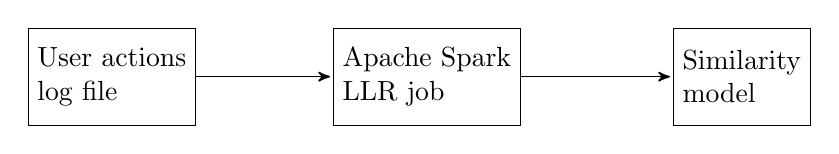
\begin{tikzpicture}[node distance=40mm,
data/.style={
rectangle,
draw,
thin,
minimum height=3.5em
},
to/.style={->,>=stealth',shorten >=1pt,semithick,font=\footnotesize},
]
\node (log) [data, align=left] {User actions\\log file};
\node (spark) [data,right of=log,align=left] {Apache Spark\\LLR job};
\node (model) [data,right of=spark,align=left] {Similarity\\model};
\draw[to] (log) -- (spark);
\draw[to] (spark) -- (model);
\end{tikzpicture}
\caption{The {\ttfamily spark-itemsimilarity} job of Apache Spark computes the LLR similarity based on the user behavior log file.}
\end{figure}

\subsection{Using more than one type of behavior}
\label{sec:multimodal}

Most collaborative filtering algorithms use only explicit or implicit ratings to compute similarity. Hence they only use one type of user behavior.
But we can improve the performance of the recommender engine by using multiple types of user actions. As described in section \ref{sec:inputdata} we record tag-associations. In addition to likes we can use tagging activity to compute similarity. In table \ref{tbl:llr1} we count the co-occurrence of items in user's like-action history. Instead of the like history we could use tags that are associated with items. We count the \gls{coocc} of each items pair associated the same tag.

Suppose we compute one \gls{indicatorm} based on likes $M_l$ and one based on tag associations $M_t$. And $h_l$ is a user's history of ``likes'' and $h_t$ is the user's tag history. We use both indicators to compute the recommendation vector $r$ by first calculation the matrix vector products of a indicator matrix with its corresponding history vector and then summing up the resulting vector (see equation \ref{eq:multi}).

\begin{equation}
  \label{eq:multi}
  r = h_l M_l + h_t M_t
\end{equation}

In our demo web application we use ``likes'' and tags but virtually all user actions can be used to improve the recommendations.

\subsection{Why can we use a search engine to produce \gls{topn}?}
\label{sec:relation}

The \gls{rec} uses a search engine to produce a \gls{topn}. We can deploy a search engine in order to provide recommendations because there are similarities between the computation of the \gls{topnt} and the retrieval of a ranked search result set.
 This section explains why the deployment of a search engine is suitable for the top-N recommendation task.

\subsubsection{Ranked retrieval}
A search engine enables user to search a collection of documents for specified keywords in a query. It returns a sorted set of documents that match the query. The result set is sorted by relevancy. The top documents are the most relevant to the query. This process is called \gls{rankedretrieval}. It does this by calculating a similarity score between each document and the query and then sorts the result by this score. The score indicates the strength of the match against the query. This is one of the main use cases where search engines shine compared to relational databases. There a row either matches a query or it does not. 

\subsubsection{Vector space model}
One way to calculate the similarity between a query $q$ and a document $d$ is to use the vector space model.
In the vector space model each document $d$ and the query $q$ are represented as vectors $\vec{v}(d)$ and $\vec{v}(q)$. The vector contains an element for each term. It maps every term $t$ of the collection to a tf-idf weight. tf-idf reflects how important a term is to a document in the collection (see \cite{Manning} for a detailed description). 
The similarity score between two items is equal to the dot product.
\begin{equation}
  \label{eq:score}
  \text{score}(d,q) = \vec{v}(d) \cdot \vec{v}(q)
\end{equation}
In order to create a ranked result set for a query $q$ the search engine computes $\text{score}(d,q)$ for all documents in the collection. We can form a matrix $C$ with the document vectors as rows. The process of scoring all document can be writen as matrix vector multiplication of $C$ and $q$. 

\begin{equation}
  \label{eq:ser}
  r = C q
\end{equation}
$r$ maps every document to a relevancy score.
This is similar to the computation of the \gls{topn} $r_u = M h_u$  described in section \ref{sec:problem}. The search engine returns documents that are similar to the query $q$. The recommender returns items that are similar to the items in the user's action history $h_u$. If we can map items to documents and the user's action history to a query we can use an existing search engine for the top-N recommendation task. This is desirable because search engines like Apache Solr are optimized for ranked retrival and they are able to process big data at scale. 

\subsubsection{How to map documents to items}

\begin{lstlisting}[caption={Item metadata and similar items are stored in Solr.},label={lst:solrdoc}]
{
    id: 1,
    title: Toy Story,
    tags:Pixar animation fantasy,
    likeindicator: 1688 1834 3893 4366 6281 33162,
    tagindicator: 10 33 41 54 55 59 66 67 72 73 80
    _version_: 1505056335358591000
}
\end{lstlisting}

The goal of our mapping is that the search engine finds the most similar items to the one in the user's action history.
The result of the search should contain a list of items. Hence we index items instead of documents.

A document in a search engine contains fields. A field contains a sequence of terms or metadata. 
Instead of finding document that contain the keywords of the query in a field we want to find items that are similar to the items in the user's recent action history. Therefore we replace the terms (words in free text) with item-id's that are similar to the item represented by the document. 

Figure \ref{lst:solrdoc} shows an example entry of a movie item formated in JSON. The indicator fields \verb|likeindicator| and \verb|tagindicator| contain movie ID's of similar movies. In addition to the indicators, the entry contains metadata about the item. These fields can be used to retrieve items by metadata, such as title or genre.

A search engine using the vector space model will use document vectors with tf-idf values to compute the score of a match. Tf-idf will mitigate popular items which is desirable but but it only accounts for the occurence of a term in a text. With the proposed mapping the term frequency of indicator ID's will be 1 or 0. We want to have some way to include the \gls{llr} ratios to boost items that have a high similarity to the item represented by the document. In order to include the similarity metric among items described in section \ref{sec:llr} we have to weight the tf-idf values in the document vector with the \gls{llr} ratios. This is the reason why we can't use a search engine out of the box without extending it's scoring function.
We have to replace the document vector with rows of the \gls{indicatorm} $M$. 

\subsubsection{Composing the query}
We store items with metadata and the corresponding similar items as a document in the search engine. To get a \gls{topn} we query the search engine with items from the user's action history $h$. The search engine will transform the item in the query to the corresponding document vector. Then it will find all items that have those recent history items as indicators. The more items the query $h$ and an item have in common the higher the similarity score. Hence we get ranked list with the most similar items on top. Table \ref{tbl:comparison} shows the mapping.

\begin{table}
\begin{center}
\begin{tabular}{lll}
 search engine & \gls{rec}\\ \hline
  document & item\\ 
 field & indicator \\
 term & indicator id    \\
 query & user's action history \\
\end{tabular}
\end{center}
\caption{We can map document, fields, term and query to the recommender equivalents. A search engine is similar to a recommender. We use the user'action history as query to find items in the collection that have those recent history items as indicators. }
\label{tbl:comparison}
\end{table}

Note that we can emulate different recommendation engines by using different queries.
\begin{itemize}
\item If the query is composed with the user's action history we use collaborative filtering with an itembased approach.
\item We can use a single item $i$ as query and get back all similar items. For instance, a top-N list of items retrieved with this query can be placed on a description page of item $i$ with the title ``Customers Who Liked This Item Also Liked''. This is a non-personalized approach.
\item We can use user profile information in the query. If the user profile contains information about the user's favorite movie genre or favourite regiseur and the search engine has index the corresponding metadata we retrieve a scored search result with respect to the fields genre and regiseur. This would be a content based approach.
\end{itemize}

\subsubsection{Implementation}
\label{sec:solrimpl}
We deploy the search engine Apache Solr in our demo webapplication. Simply put, Solr is a Web API for Apache Lucene, an open source information retrieval software library. 

In order to use the precomputed \gls{llr} ratios of the \glspl{coocc} we need a way to store them per term and per document. Lucene provides this functionality with the \emph{playloads} feature. Payloads enable an application to store an arbitrary byte array for every term during indexing \cite{McCandless}.

Unfortunatly the feature is only implemented in Lucence, not in Solr. But we can extend Solr to use the Java classes that deal with payloads.

First we need to define a new fieldtype in the schema.xml of our Solr configuration. Fields of this type contain terms with an added payload.
To index the similarity value we define a custom fieltype that uses Lucene's DelimitedPayloadTokenFilter to extract a payload from every term. 

\begin{lstlisting}[caption={Fieldtype definition for field with payload.}]
<fieldtype name="payloads" class="solr.TextField" >
 <analyzer>
  <tokenizer class="solr.WhitespaceTokenizerFactory"/>
   <filter class="DelimitedPayloadTokenFilterFactory" />
 </analyzer>
</fieldtype>
\end{lstlisting}
The default delimiter is the pipe symbol. With this fieldtype we can add payloads to terms in document be attaching a number to the term string.
\begin{verbatim}
23|0.9
\end{verbatim}
In this example \verb|23| is an item-id and \verb|0.9| is the similiarity value to the corresponding item.

After we stored the payload within the index we need a way to score a document match according the payload.
Solr uses per default the vector space model to compute the score between a document $d$ and a query $q$. It only considers terms $t$ that appear in the query $q$. The tf-idf weight is multiplied by a boosting factor for a term $t$ \cite{grainger}.  
\begin{equation}
\label{eq:solrsim}
\text{score}(q,d) = \sum_{t \in q} \text{tf-idf}(t,d) \cdot \text{boost}(t)
\end{equation}

In order to use the payload values in the ranked retrieval process we have to extend Solr with our own Query Component. 

We can add a custom Query Component by implementing a \verb|QParserPlugin|. The implementation just returns the \verb|PayloadTermQuery|. \verb|PayloadTermQuery| matches all documents containing the specifed term and than applies a scoring factor based on the payload that is stored with each term.

In addition we have to override the method \verb|scorePayload| of the \\ \verb|DefaultSimilarity| class. \verb|PayloadTermQuery| will call \verb|scorePayload| to determine the payload of an item and then it multiplies the td-idf weights with the corresponding payload. We have to tell Solr to use our custom Query Component and the new \verb|PayloadSimilarity| by adding the following entries to the solrconfig.xml.

\begin{lstlisting}
<similarity class="ch.hsr.solrpayload.PayloadSimilarityFactory">
<queryParser name="payloadparser" 
   class="ch.hsr.solrpayload.PayloadParser" />
\end{lstlisting}
  
Solr will load the implementations from it's \verb|lib| directory if we package them Java jar archive.

\begin{figure}
  \centering
\begin{tikzpicture}
  \begin{axis}[
    title=evaluation of LLR threshold,
    xlabel=threshold,
    ylabel=Precision/Recall,
    width=10cm,
    ]
\addplot table {thresholdp.dat};
\addplot table {thresholdr.dat};

  \end{axis}
\end{tikzpicture}
\caption{The precision and recall at 10 for the MovieLens data set is measured as a function of the similarity threshold. Items with a small similarity value do not contribute to the performance. The best performance is archieved by only adding items with a \gls{llr} ratio above 0.9.}
\label{fig:threshold}
\end{figure}

In our demo web application we only add items above a given \gls{llr} ratio threshold to the index of the search engine. If we add items with a small similarity to the indicator fields the precision and recall decline. The evaluation in figure \ref{fig:threshold}shows that the we archieve the best performance with a threshold of 0.9.

An alternative to the use of payloads is to ignore similarities values once we removed the item below threshold from the index. In that case the scoring of a document only depends on the tf-idf weight. Only add items above a threshold to the indicator fields. This approach is easier to deploy but it doesn't account for different similaries. 

\section{Integration}
\label{sec:integration}

This section describes how we integrate the components described in section \ref{sec:design}. The section is divided according the online and offline parts of the \gls{rec}.

\begin{description}
\item[Offline learning] In this part the systems uses the stored histories of user behavior to compute the \gls{llr} ratios of the \gls{coocc} among items. Then it updates all items in the in the NoSQL database/search engine Apache Solr. We use similar items as indicators and store the \gls{llr} ratios from the previous step as payloads. This task takes serveral minutes but the duration does not impact the user experience hence it can be executed overnight. 
\item[Online logging and recommendation] The online part of the system records user activities used in the similarity analysis and creates personalized \gls{topn} if requested. If it receives a requerst for a recommendation list it constructs a query from the user history $h_u$. Then it uses the query to get a ranked list of items that are likely appealing to the user $u$. It removes all item's the user already knows and present the list as recommendation. In order to a  provide smooth user experience the top-N recommendation task should not take longer than a second.
\end{description}

To store the user's activity we used a sqlite3 database because it's easy to deploy in a development environment and we can use existing interfaces for Java and Python to update and retrieve data. 

First we insert a document for every item into Solr. The documents contain the metadata like (title, genre, tags, etc). The offline learning step will only update the indicator fields for every item.

\subsection{Offline learning}
\label{sec:offline}

\begin{figure}
\centering
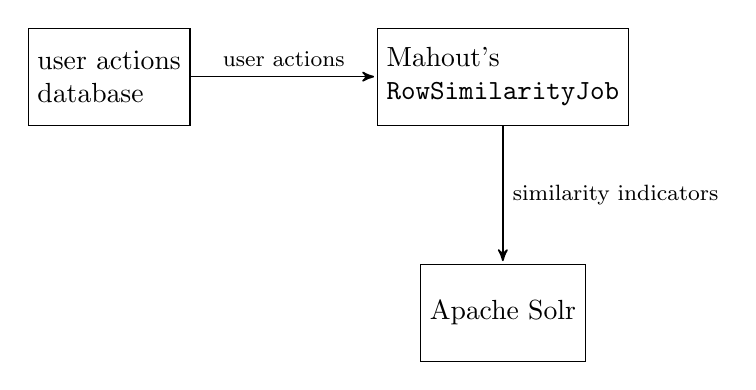
\begin{tikzpicture}[node distance=20mm,
data/.style={
rectangle,
draw,
thin,
minimum height=3.5em
},
to/.style={->,>=stealth',shorten >=1pt,semithick,font=\footnotesize},]

\node (history) [data,align=left] {user actions\\database};
\node (spark) [data,right of=history,node distance=50mm, align=left] {Mahout's \\\verb|RowSimilarityJob|};
\node (solr) [data,below of=spark,node distance=3cm] {Apache Solr};
\draw[to] (history) -- node[midway,above]{user actions} (spark);
\draw[to] (spark) -- node[midway,right] {similarity indicators} (solr);
\end{tikzpicture}
\caption{The offline learning part uses user log files stored in a sqlite3 database to compute the similarities with Mahout's {\ttfamily RowSimilarityJob}. The result is loaded into Solr.}
\label{fig:offline}
\end{figure}

The offline learning part is done in three steps.

\begin{enumerate}
\item Read the recorded \glspl{useraction} from a sqlite3 database and convert it as required by \verb|RowSimilarityJob|.
\item Generate \glspl{indicator} with Mahout's \verb|RowSimilarityJob| that connects to a Apache Spark server.
\item Use the output of \verb|RowSimilarityJob| to update the indicator fields of all items stored in Solr.
\end{enumerate}

The computation of similarities and update of Solr involves a lot transforming data from one format to another. We have implemented a command line tool, \verb|updatesearchengine|, that executes all three steps. 

\subsection{Online recommendation}
\label{sec:online}

The generation of a top-N recommendation list can be divided into 4 step. The process is illustrated in figure \ref{fig:topn}.

\begin{enumerate}
\item User requests top-N recommendation list.
\item Look up the user's action history $h_u$.
\item Query the search engine.
\item Process the search result and format a JSON response.
\end{enumerate}

These steps are implemented in the web application with a few lines of code. The the heavy lifting is done by the search engine.

First the web browser requests a top-N recommendation list for user $u$. In our demo application the web server provides a REST API. A authenticated user can issue a \verb|GET| request to the path \verb|/topn| in order to get the list. 
When the web server receives a request it looks up the action history $h_u$ for user $u$ in the user action database. $h_u$ can contain multiple types of user behavior. In our demo application the web server retrieves a list of items the user liked in the past and a list of items the user tagged. In order to retrieve all actions that belong to user $u$ the user activity is stored in a relational database.
Then the web server forms a Solr query with the recent users actions, and sends Solr a HTTP request that contains the query as \verb|q| parameter. For instance the following string shows the \verb|q| parameter for a HTTP request that uses recent user likes and tag activity.
\begin{verbatim}
q=likeindicator:1688 1834 3893 AND tagindicator:10 33 41 54 55 
\end{verbatim}
Solr returns a raw ranked result list. 

To produce a top-N recommendation list the web server uses the user history $h_u$ again to removes all item already known to the user. Then it formats the data as JSON and presents the user a top-N recommendation list. In addition we could apply business logic that adjusts which items are shown. For instance, we can promote particular items or we could remove out-of-stock items.

Listing \ref{lst:topn} shows the Scala code that does the filtering and formatting.
\verb|solrResponse| is a \verb|Iterable| that yields the ranked result set from Solr. \verb|history| is a list of all items the user liked or tagged. \verb|toJson| takes an \verb|Writes[T]| as implicit parameter. Hence we transform \verb|SolrDocument| by implementing \verb|Writes[SolrDocument]|.

\begin{lstlisting}[caption={The web server removes items already known and formats the the items in JSON},label={lst:topn}]
def itemIsKnown(x: SolrDocument) =
      history.contains(x.getFieldValue("id").toString())
      
val unknownItems = solrResponse.filter {!itemIsKnown(_)}
Ok(Json.toJson(unknownItems))
\end{lstlisting}

\begin{figure}
\centering
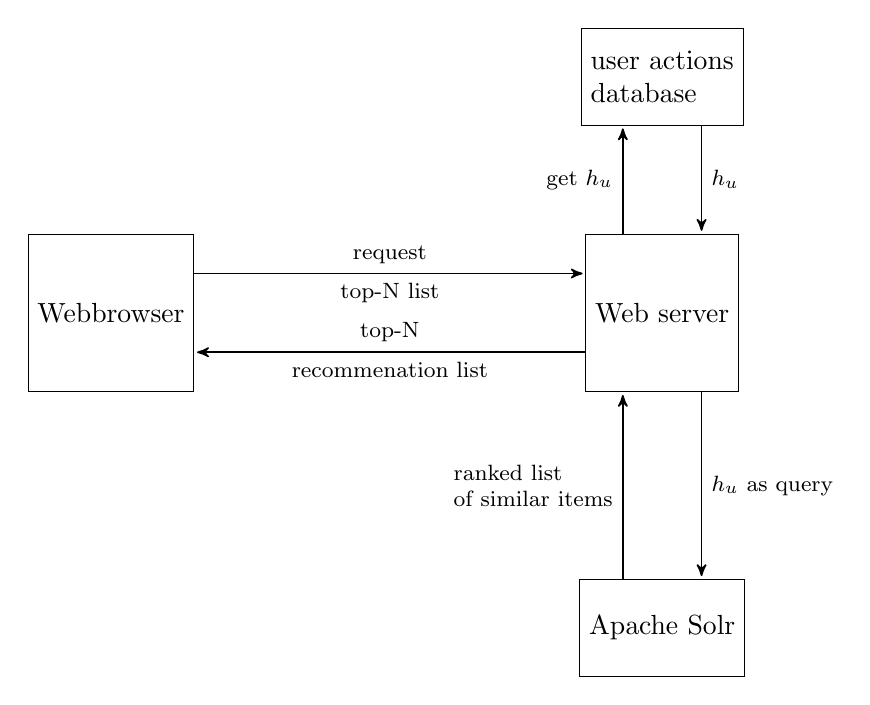
\begin{tikzpicture}[node distance=20mm,thick,
data/.style={
rectangle,
draw,
thin,
minimum height=3.5em
},
to/.style={->,>=stealth',shorten >=1pt,semithick,font=\footnotesize},]
]

\node (web) [data, minimum height=2cm] {Web server};
\node (log) [data,above of = web,align=left,node distance=30mm] {user actions\\database};
\node (browser) [data,left of=web,node distance=7 cm,minimum height=2cm] {Webbrowser};
\node (solr) [data,below of=web,node distance=4 cm] {Apache Solr};
\draw[to] ([yshift=0.5 cm]browser.east) -- node[midway,above]{request} node[midway,below]{top-N list} ([yshift=0.5 cm]web.west);
\draw[to] ([yshift=-0.5 cm]web.west) -- node[midway,above]{top-N} node[midway,below]{recommenation list} ([yshift=-0.5 cm]browser.east);
\draw[to] ([xshift=-0.5 cm]web.north) -- node[midway,left]{get $h_u$} ([xshift=-0.5 cm]log.south);
\draw[to] ([xshift=0.5 cm]log.south) -- node[midway,right]{$h_u$}([xshift=0.5 cm]web.north);
\draw[to] ([xshift=0.5 cm]web.south) -- node[midway,right]{$h_u$ as query}([xshift=0.5 cm]solr.north);
\draw[to] ([xshift=-0.5 cm]solr.north) -- node[midway,left,align=left]{ranked list\\of similar items } ([xshift=-0.5 cm]web.south);
\end{tikzpicture}
\caption{To produce a top-N recommendation list the web browser requests a top-N recommendation list for user $u$. The webserver looks up the action history $h_u$ for user $u$ in the user action database. Then the webserver forms a Solr query with the recent users actions and sends it to Solr. Solr returns a raw ranked result list to the web server. The webserver removes all item already known to the user formats the data to JSON and presents the user a top-N recommendation list. }
\label{fig:topn}
\end{figure}
%-- node[midway,above] {post user actions}
\section{Evaluation}
\label{sec:evaluation}

This section describes the evaluation process and presents the results of the evaluation.

Evaluation is important because:
\begin{itemize}
  \item It allows us to decide if the quality of the recommender engine archives the desired results. 
  \item We are able to compare the recommender
  \item Evaluation allows us to adjust the parameters in order to get better results.
  \item It allows us to compare different recommender techniques.
\end{itemize}


Most commonly accepted evaluation measure for recommender systems is the Mean Average Error or Root Mean Squared Error of the predicted ratings and the actual one \cite{Ricci}.

The recommender engine discussed in this article does not estimate preference values in order to produce recommendations. It presents a ordered list of $n$ recommendations.   The list is ordered from best to worst recommendation. It produces a Top-N list of recommendations. The recommenders classifies recommendable items. If we look at the recommender problem as a classification problem we can make use of precision and recall. Precision and Recall are two information retrieval concepts. We provide a brief summary here to each of these measures.

Precision and recall depend on the following measures.
\begin{description}
\item[True positive (TP)] Number of items classified as recommendable or relevant that is truly of interest to the user.
\item[True negatives (TN)] Number of instances not contained in the recommendation list (classified as irrelevant) and that in fact are not of interest to the user.
\item[False positives (FP)] Number of instances recommended but are not relevant to the user.
\item[False negatives (FN)] Number of instances not shown in the recommendation list but that in fact are relevant to the user.
\end{description}


\begin{figure}
\centering
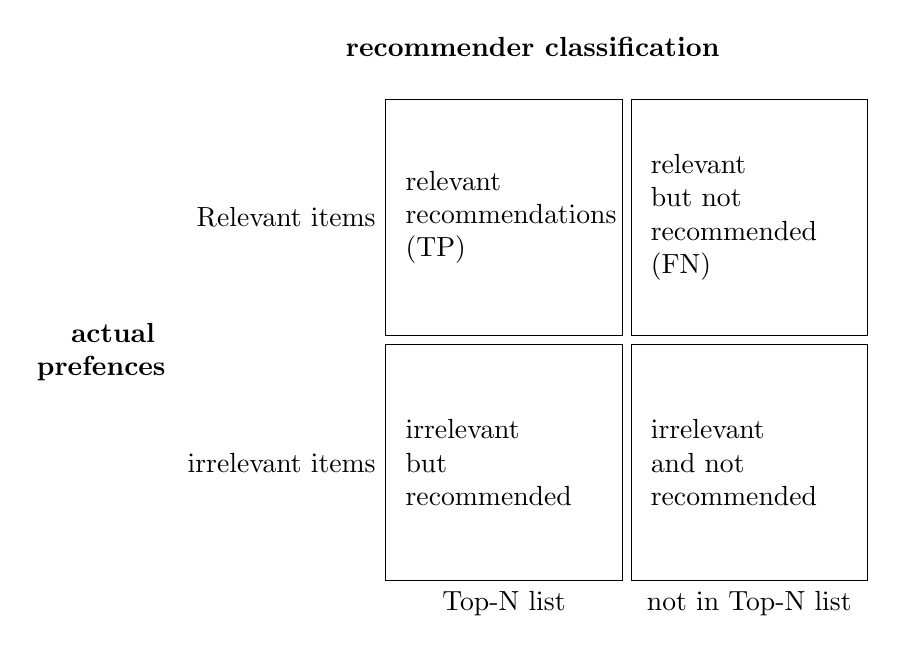
\begin{tikzpicture}[
box/.style={draw,rectangle,minimum size=3cm,text width=2.5cm,align=left}]
\matrix (conmat) [row sep=.1cm,column sep=.1cm] {
\node (tpos) [box,
    label=left:Relevant items,
    label=above:,
    ] {relevant \\ recommendations \\ (TP)};
&
\node (fneg) [box,
    label=above:,
    label=above right:,
    label=right:] {relevant\\ but not \\recommended\\(FN)};
\\
\node (fpos) [box,
    label=left:irrelevant items,
    label=below left:,
    label=below:Top-N list] {irrelevant \\but\\recommended};
&
\node (tneg) [box,
    label=right:,
    label=below:not in Top-N list] {irrelevant\\and not\\recommended};
\\
};
\node [left=.05cm of conmat,text width=1.5cm,align=right] {\textbf{actual \\ prefences}};
\node [above=.05cm of conmat] {\textbf{recommender classification}};
\end{tikzpicture}
\caption{Confusion matrix for top-N recommendation task}
\label{fig:confusionmatrix}
\end{figure}

Figure \ref{fig:confusionmatrix} visualizes the measures used for precision and recall. This table is called confusion matrix or contingency table. 

\subsection{Precision and Recall}
\label{sec:precision}

\begin{description}
\item[Precision] Precision is the proportion of items in the top-N list of recommendatoins that are relevant \cite{Manning}.
  \begin{equation}
    \label{eq:precision}
    \text{Precision} = \frac{\text{number relevant items recommended}}{\text{size of the recommendation list}}
  \end{equation}
We can formulate this with the measures from the confusion matrix.
  \begin{equation}
    \label{eq:recallcm}
    \text{Precision} = TP/(TP+FP)
  \end{equation}

 Suppose the recommender create a list of 5 items. If 3 items are relevant recommendations then the precision is $3/5$. 
Precsion only considers the accuracy of the recommendation list and not the comprehensiveness of the result.

\item[Recall] Recall is the proportion of relevant items that appear in the recommendation result. 
  \begin{equation}
    \label{eq:recall}
    \text{Recall} = \frac{\text{number relevant items recommended}}{\text{relevant items}}
  \end{equation}
  \begin{equation}
    \label{eq:recallcm}
    \text{Recall} = TP/(TP+FN)
  \end{equation}
Suppose there are 9 relevant recommendations. If the recommender results contains 3 of these relevant recommendations then the recall is 3/9.

Note that recall should not used without precision. We could build a recommender with perfect recall by recommending all items.
\end{description}

\subsubsection{Implementation}
\label{sec:irimpl}

Listing \ref{lst:irstats} shows the implementation of precision and recall. 
The variable \verb|rec| contains an object of type \verb|Recommender|. \verb|Recommender| provides the method \verb|recommend|. \verb|recommend| takes the ID of th active user and the size $N$ of the top-N list as parameters. The argument |verb|topNsize| corresponds to $TP+FP$. It returns a top-N list for the active user. 

The variable \verb|relevantItemIDs| contains a list with relevant items for the active user.

We count how many items in the top-N list are also in the list \verb|relevantItems| and assign the result in \verb|relevantItemsRetrieved|. \verb|relevantItemsRetrieved| corresponds to the $TP$ value. In order or compute precision or recall we divide \verb|relevantItemsRetrieved| by \verb|topNsize| or the size of the collection\\ \verb|relevantItems|.

\begin{lstlisting}[caption=Implementation of precision and recall,label=lst:irstats]
double precision = 0;
double recall = 0;
int relevantItemsRetrieved = 0;

List<RecommendedItem> recItems = rec.recommend(userID, topNsize);
   for (RecommendedItem recItem : reItems) {
	if (relevantItem.contains(recItem.getItemID())){
			relevantItemsRetrieved++;
	}
   }

// Precision
int numRecommendedItems = reItems.size();
precision = ((double) relevantItemsRetrieved / (double) topNsize);
		      
// Recall
recall =  relevantItemsRetrieved / (double) relevantItems.size());
		      
\end{lstlisting}


\subsubsection{Testing Methodology}
\label{sec:relevant}

If we want to evaluate a recommender, we have to define, what is a relevant item for the active user. For the user a relevant item is one that he does not know and he would like (or purchase). Those items are unknown at the time of the recommendation. Relevancy depends on the goal of the recommender. For example, an item is relevant if the user would give it a high rating or if he would purchase the item.

Unfortunatly we do not know how a user likes some new item in the future.
But we can simulate the prefencences of the future by setting aside a small part of the real data set as test data. We split the collected input data into as follows:


We get the all ratings of user $u$. We sort these rating according the rating value. Then we select the top $N$ items $T$ from the sorted list. Items in $T$ have a high rating and we assume that it is relevant to the user $u$.
All ratings in $T$ are removed from the overall input set. The remaining preferences form the training data set $M$. 

In order to measure precision and recall we first train the recommender with the data in $M$.

We determine the top the top $N$ preferences for each user. Then we remove these values from the input data set. The resulting set is the training data set. We use this set to train the recommender engine. For instance, if we evaluate a co-occurence based recommender we compute indicator matrix from section \ref{sec:llr} with this set.

The removed entries form the test data set. Items in the test data set are the relevant items. 
For example, if $n$ is 5 this would mean precision is evaluated by removing the top 5 preferences for a user and then finding the percentage of those 5 items included in the top 5 recommendations for that user. 

The evaluatuation of the recommender can be devided into several steps:
\begin{enumerate}
\item  Compute the indicator matrix with the training set.
\item Update the search engine with the similarity values.
\item Generate a list of recommendations $r_u$ for each user.
\item Measure the precision and recall for all generated recommendations list $r$ and return the mean value.
\end{enumerate}

The evaluation process has the following parameters:
\begin{description}
\item[Size of the result] The number of recommendations to consider. The length of the recommendation list.
\item[Relevance threshold] Determines if an item is relevant or not.
\end{description}

\pgfplotsset{width=7cm}
\begin{figure}
  \centering
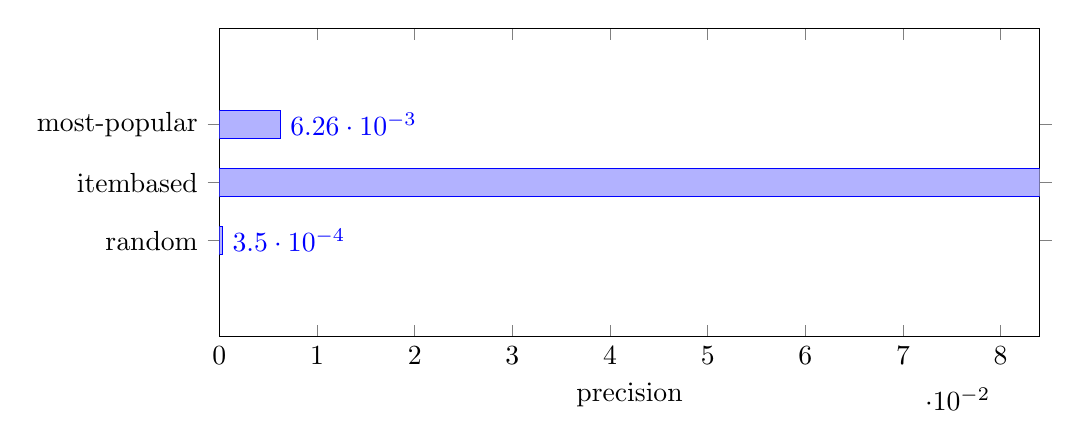
\begin{tikzpicture}
\begin{axis}[
xbar,
xmin=0,
xmax=0.084,
width=12cm,
height=5.5cm,
enlarge y limits=0.83,
xlabel={precision},
symbolic y coords={random, itembased,most-popular},
ytick=data,
nodes near coords,
nodes near coords align={horizontal},
]

\addplot coordinates {(0.00035,random) (0.00626,most-popular) (0.0864,itembased) };
\end{axis}
\end{tikzpicture} 
  \caption{Precision and recall comparison of an random generated recommendations and recommendations of itembased recommonder. The number of recommended items is 15}
  \label{fig:precisionrecallvalues}
\end{figure}

In order to get a feel what values of precision an recall to excpect we measured an itembased recommender and random generated recommendion list \cite{jannach11}.
An itembased recommender engine archives an average precision value of 0.00358. This seems a small value but if we return randomly generated recommendations we get a precision of 0.00095. Hence an itembased recommender improves the precision with a factor of 3. Figure \ref{fig:precisionrecallvalues} shows the comparison of the two measurements. We used the movielens data set for this evaluation (see section \ref{sec:dataset}).

Precision and recall has the following paramters
\begin{itemize}
\item Size of the recommendation list $N$. How many recommended items are expected. The number of items retrieved. True positives and false positives.
\item What are relevant items. Relevant items could be a threshhold in preference. Or it could be a function that return user's average preference value plus one standard deviation.
\end{itemize}

\subsection{Mahouts Evaluator}
\label{sec:mahouteval}

The library Apache Mahout provides a method to evaluate precision and recall. It is implemented in 
 \verb|GenericRecommenderIRStatsEvaluator| in the package \verb|org.apache.mahout.cf.taste.impl.eval|. The problem with this method is that the number of retrieved document $n$ is equal to the number of relevant documents and if a user has many items above threshold  \verb|GenericRecommenderIRStatsEvaluator| takes only $n$ of those. It's desirable to parameterize the definition of relevant items and number of retrieved items independently.

\begin{quote}
For each user, these implementation determine the top n preferences, then evaluate the IR statistics based on a DataModel that does not have these values. This number n is the "at" value, as in "precision at 5". For example, this would mean precision evaluated by removing the top 5 preferences for a user and then finding the percentage of those 5 items included in the top 5 recommendations for that user. 
\end{quote}

\begin{quote}
  items whose preference value is at least this value are considered "relevant" for the purposes of computations
\end{quote}

What is the impact of the parameter relevanceThreshold. According to the class description the relevant items are the users top n preferences. 

According to the description of the parameter relevanceThreshold the items whose preference is at least the threshhold are relevant. 



\subsection{Dataset}
\label{sec:dataset}

This dataset used in this project describes rating and free-text tagging activity from MovieLens, a movie recommendation service \cite{movielensdata}.
MovieLens data sets were collected by the GroupLens Research Project at the University of Minnesota.

The data was collected through the MovieLens web site (movielens.umn.edu) during the seven-month period from September 19th, 1997 through April 22nd, 1998 \cite{movielensdata}.
 
This data set consists of:
\begin{itemize}
\item 100,000 ratings. The ratings are numbers from 1 to 5. A rating is made by one user to one movie at a specific time. Each line of this file after the header row represents one rating of one movie by one user, and has the following format:
\begin{verbatim}
userId,movieId,rating,timestamp.
\end{verbatim}
\item 943 users. Each user has rated at least 20 movies
\item 1682 movies. Movies are categorized in genres. 
\item 2488 tag appliciations. A tag is applied by one user to one movie at a specific time. Tags are user-generated metadata about movies. Each tag is typically a single word or short phrase. The meaning, value, and purpose of a particular tag is determined by each user. All tags are contained in the file $tags.csv$. Each line of this file after the header row represents one tag applied to one movie by one user, and has the following format:
\begin{verbatim}
userId,movieId,tag,timestamp
\end{verbatim}
\end{itemize}

Time in the the ratings and tags set is formatted as timestamps that represends seconds since midnight Coordinated Universal Time (UTC) of January 1, 1970.

\subsection{Baseline Algorithm}
\label{sec:baselinealgorithm}

We compare the co-occurence based recommender to an item-based recommender. This section will give a brief description of item based recommenders.

\subsection{Results}
\label{sec:results}
\begin{figure}
  \centering
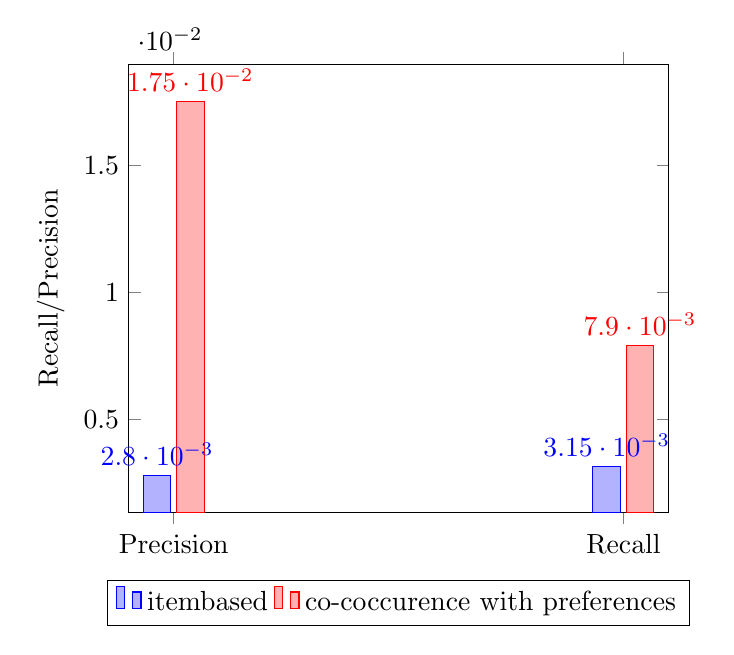
\begin{tikzpicture}
\begin{axis}[
ybar,
%enlargelimits=0.45,
legend style={at={(0.5,-0.15)},
anchor=north,legend columns=-1},
ylabel={Recall/Precision},
symbolic x coords={Precision,Recall},
xtick=data,
%ybar=5pt,% configures ‘bar shift’
%bar width=9pt,
nodes near coords,
nodes near coords align={vertical},
]
\addplot coordinates {(Precision,0.0028) (Recall,0.00315)}; 
\addplot coordinates {(Precision,0.0175) (Recall,0.0079)};

\legend{itembased,co-coccurence with preferences}
\end{axis}
\end{tikzpicture} 
  \caption{Precision and recall comparison of an item-itembased recommonder and the cooccurrence based. The result setsize is 10}
  \label{fig:results}
\end{figure}

\section{Conclusion}
\label{sec:conclusion}

We have built a prototype of a \gls{multimodal} \gls{rec} with a search engine according to the suggestions of \cite{Dunning14}. 
This approach simplifies the development process and lowers the entry barrier for developer without a strong mathematical background because we do not have to make descisions which algorithms or similarity metrics to choose. 

User interaction is the best clue what users want.
The design allows to use a variety of user interactions and metadata as input data. This hybrid approach improves the performance of the \gls{topnt}. Multiple \glspl{indicator} are stored in distinct field within Solr. The recommender engine can be extended with additional \glspl{indicator}.


The calculation of \gls{coocc} indicator matrix and therefore the update process of the search engine is computational expensive. Mahout's \verb|spark-itemsimilarity| job allows us to compute \gls{indicatorm} at scale.
The two part design of the \gls{rec} allows us to do the heavy lifting upfront. In return the \gls{topnt} is performed blazingly fast because Apache Solr is optimized for text retrieval queries. 

A large amount of work was required to convert formats between the user history database, the Apache Mahout and Apache Solr. 

The proposed design did not described the inclusion of item similarity values in the search engine. We used the payload mechanism of Apache Lucene to weight indicator with the corresponding similatity value.

Unfortunatly \cite{Dunning14} does not descibe an evaluation method for the proposed design. We evaluated the recommnender with the accuracy metrics precision and recall. The usefulness of these metrics depends on the definition of relevant items. We defined items that the user has given a high rating as relevant. The evaluation method used in this report penalizes items that the user never has rated or even seen. 

Another problem with precision and recall emerges when the preferences are Boolaen data, like in the demo application, because we can not pick the $N$ best rated items and have to select them at random. For this reason we used the MovieLens data set that contains preference values and simulated user actions.

The evaluation results of the co-occurence based recommender are not overwhelming. Compared to the \gls{itembased} recommender the increase of quality is small. But the evaluation method only considers items that the users already liked as relevant. We do not know how usefull a recommendation for an individual user is. It could be that the co-occurence based recommender is suggesting items that the user never has seen and that are desirable for the user.

The system may be improved throug the use of 
\begin{description}
\item[Dithering] 
\item[Anti-flood] 
\item[Cross-coooccurence]
\end{description}
dithering.



\appendix

\section{Installation Guide}
This section describes the usage of the various scipts and the demo web application created during the project.
\subsection{Tools, libraries and frameworks}
The web application demo and the evaluator were developed on a Ubuntu 15.04. 
The following software was used to build the evaluator, the search engine update job and the web application. We assume that they are installed on the user's computer.
\begin{itemize}
\item JVM 1.8.45 OpenJDK. Solr, Spark and Play run on the JVM.
\item Scala Compiler 2.11.7. The web application is written in Scala.
\item sbt 0.13.8 (Scala Build Tool) . The web application can be build with sbt.
\item Maven 3.19 (Java build tool). Maven was used to build Spark and the evaluator.
\item Solr version 4.7.2
\item Spark version 1.1.1. The Mahout shell job \verb|spark-itemsimiliarity| uses Spark to compute LLR ratios.
\item Play version 2.4. We used the Play framework because it runs on the JVM and we can use the Solr Client Library in the web server.
\item AngularJS. Javascript Framework. Used for WebGUI.
\item Mahout 0.10.0. The machine learning library Apache Mahout is used to compute the LLR ratios and for the evaluation.
\item sqlite3 3.8.7.4. We use sqlite3 because there are JDBC drivers and a python interface.
\item python 2.7.9. Python is used to transform the date from sqlite3 to the input format of Apache Spark.
\end{itemize}

\subsection{Starting Apache Solr}
\label{sec:startsolr}
The demo web application and the update script depend on a running Solr instance.
To start a Solr instance with the movielens core run
\begin{verbatim}
java -jar start.jar
\end{verbatim}
in the directory \verb|solr|.
This will start a Jetty instance that is listening on port 8983. To access the administration web interface visit \verb|http://localhost:8983/solr/| with a web browser.

\subsection{Start the demo web application}

The demo web application requires a running Solr instance. Make sure you executed the steps described in section \ref{sec:startsolr} before you start the web application. The Solr instance that the web application will use can be configured in the file \verb|movierecommender/conf/application.conf|. The URL of the Solr instance can be set with the key \verb|solr.url|. For example
\begin{verbatim}
solr.url="http://localhost:8983/solr/movielens"
\end{verbatim}

To run the demo web application change to the directory \verb|movierecommender| and execute the sbt command \verb|sbt run|.

\subsection{Indicator computation- and update script}
In order to run the Python script \verb|updateSolr.py| the following environment is required.
\begin{itemize}
\item Apache Mahout shell is installed.
\item sqlite3 client is installed (can be installed with \verb|apt-get install sqlite3| on a system with Aptitude). 
\item The script requires a running spark instance. Apache Spark can be downloaded from \url{http://spark.apache.org/downloads.html}. Spark contains a shell script \verb|sbin/start-master.sh| to start a master node.
\item A running Solr instance with the movielens core. The solr directory contains the \verb|start.jar| application. To start a Solr instance with the movielens core run \verb|java -jar start.jar|.
\end{itemize}

In addition the following environment variables must be set:
\begin{description}
\item[MAHOUT\_HOME] Directory of the Mahout installation.
\item[JAVA\_HOME] JDK installation directory.
\item[SPARK\_HOME] Directory of the Spark installation.
\item[MASTER] Url of the spark master node (e.g. spark://localhost:7077).
\end{description}

The script takes two parameters. The file of the sqlite3 database and the URL of the Solr instance. For example:
\begin{verbatim}
python updateSolr.py movie.db http://localhost:8983/solr/movielens
\end{verbatim}

The shell script \verb|startUpdateSolr.sh| will run this script with an example configuration.

\subsection{Running the evaluation}

The directory \verb|evaluator| contains the evaluation program descibed in section \ref{sec:evaluation}. In order to build it change to the directory \verb|evaluator| and run the maven command
\begin{verbatim}
mvn clean compile assembly:single
\end{verbatim}
This creates an executable jar archive. To start the evaluation run 
\begin{verbatim}
java -jar target/evaluator-0.0.1-jar-with-dependencies.jar
\end{verbatim}

The program expects the following parameters:
\begin{description}
\item[precisionat] Set the size $N$ of the top-N list.
\item[Solr instance URL] URL of the Solr instance.
\item[Ratings filepath] File path of a CSV file that contains user ratings
\item[Tags filepath] File path of a CSV file that contains tag - item interactions.
\end{description}

The shell script \verb|startevaluator.sh| starts an example evaluation.

\section{Source code listings}
\label{sec:listings}

\begin{lstlisting}[caption={To simulate the user action ``like'' we extract all ratings equal or above a score of 4.0 and use the result as training set},label={lst:pref2like}]
 public GenericBooleanPrefDataModel pref2like(DataModel dataModel,
	float threshold) {
	try {
	FastByIDMap<FastIDSet> userlikes = new FastByIDMap<FastIDSet>(
					dataModel.getNumUsers());
	LongPrimitiveIterator iter = dataModel.getUserIDs();
	while (iter.hasNext()) {
          long userid = iter.nextLong();
          PreferenceArray prefs = dataModel
		.getPreferencesFromUser(userid);
          FastIDSet ids = new FastIDSet(prefs.length());
          for (Preference p : prefs) {
		if (p.getValue() >= threshold) {
                  ids.add(p.getItemID());
			}
		}
	userlikes.put(userid, ids);
	}
    return new GenericBooleanPrefDataModel(userlikes);
\end{lstlisting}


\begin{lstlisting}[ caption={Implementation of top popular recommender}]
Map<Long, Integer> item2pop = new HashMap<Long, Integer>();
LongPrimitiveIterator iter = dataModel.getUserIDs();
while (iter.hasNext()) {
PreferenceArray prefs = dataModel.getPreferencesFromUser(iter
	.nextLong());
for (int i = 0; i < prefs.length(); i++) {
	Integer counter = item2pop.get(prefs.getItemID(i));
	if (counter == null) {
		item2pop.put(prefs.getItemID(i), 1);
	} else {
		item2pop.put(prefs.getItemID(i), counter + 1);
	}
      }
}
List<RecommendedItem> popitems = transfom2list(item2pop);
Collections.sort(itemidcounter, new RecommenderItemComparator()); 
return popitems
\end{lstlisting}


\begin{lstlisting}[caption={To transform SolrDocument to JSON Object we define a implicit definition of Writes[SolrDocment].}, label={lst:writes}]
implicit val solrdocWrites = new Writes[SolrDocument] {
  def writes(solrdoc: SolrDocument) = Json.obj(
     "title" -> solrdoc.getFieldValue("title").toString().filter { _ != '[' }.filter { ']' != _ },
     "id" -> solrdoc.getFieldValue("id").toString().toLong)
}  
\end{lstlisting}

\section{Apache Solr}
\label{sec:solr}

Apache Solr is a search engine that is optimized to search large volumes of text-centric data and return results sorted by relevance. It is built on Apache Lucene, an information retrieval library \cite{grainger}. Solr stores the documents in a flat structure and we can search for terms in the documents. It provides a HTTP API for all interactions, like quering, updating e.t.c.

The reason why we deploy a search engine in order to make recommendations is that Solr scores documents based on the presence of query terms in the document similar to a recommendations engine based on the presence of indicator.

Another reason why we deploy a search engine is that the application is read-dominant. The recommender will query the data far more often than it will create new documents or update the indicators. Solr is optimized to for executing queries as opposed to storing data.

\section{Apache Mahout}
\label{sec:mahout}

Apache mahout is a top-level Apache project that provide implementations of collaborative filtering algorithms among other machine learning techniques. The development began in 2008 \cite{Owen}. It provides server Apache Spark jobs in order to process large amount of data. We used it because it's Spark support and because it's well documented.
Mahout provides a large set of recommender algorithms. And it is easy to evaluate and compare several algorithms on a specific dataset.

\subsection{Data representation}
\label{sec:datarepresentation}

Apache Mahout uses it's own data structures to store and access preference data. Mahout provides it's own map implementation \verb|FastByIDMap|. Keys in \verb|FastByIDMap| are long primitives instead of java objects. In addition \verb|FastByIDMap| has no additional \verb|Map.Entry| object per entry. The avoidance of java object saves memory. Depending on the implementation of the JVM a java object allocates about 28 bytes of memory. \verb|FastByIDMap| consumes about 28 bytes per entry, compared to about 84 byte per entry for \verb|HashMap| from \verb|java.util|.

\section{Log-likelihood ratio}
\label{sec:llrratio}
The log-likelihood metric quantifies the propability of how
unlikely it is that two items interact with the same users is due to chance. The less likely, the more similar we are.
In order to compute the \gls{llr} ratio of the \gls{coocc} among item $A$ and item $B$ we have to count how many users interacted both with $A$ and $B$, how many users interacted with $A$ without interacting with $B$, how many users interacted with $B$ without interacting with $A$ and how many user interacted with none of them.

 \todo{llr contency table einfuegen und formel fuer llr}

\section{Infrastructur}
\label{sec:infrastructur}

\subsection{Webapplication}
\label{sec:web}

To start the Webapplication run:
\begin{verbatim}
sbt build 
\end{verbatim}
This assumes that the scala build tool (sbt) is installed.
\subsection{Apache Spark}
\label{sec:spark}
Apache Spark is a cluster computer framewor. It allows user programs to load data into a cluster's memory. It is well suited to machine learning algorithms \cite{Karau}.
\subsubsection{How to deploy Spark}
\label{sec:sparkdeploy}

To run \verb|spark-itemsimilarity| we have to deploy Apache Spark and and start it in standalone mode with the script \verb|start-master.sh|. Once startet the script will print a URL which we can pass the \verb|spark-itemsimilarity| job as ``master'' argument and the job can connect to the cluster. 

\section{Sample Input Data}
\label{sec:sampleinput}

\begin{lstlisting}[label=lst:sampledata]
itemid, userid, timestamp
1,101,980730861
1,102,980731380
1,103,980731926
2,101,980732037
2,103,980730408
2,104,980731766
3,101,980731282
3,102,980730769
3,103,980731208
4,102,980732235
4,103,980731417
5,101,980731745
5,102,980731621
5,103,980731417
5,104,980731208  
\end{lstlisting}


\printglossary
\bibliographystyle{plain}
\bibliography{a}
\end{document}

